\chapter{Literature Review}
% Main Gist 
% - History of FHR reactor type and why there is a renewed interest in this
%   reactor type (start ups, labs etc.)
% - Past applications of AI to nuclear reactor design. 
% Structure 
% - Fluoride-Salt-Cooled High-Temperature Reactor (why salt cooled triso fuelled 
%   reactors are cool)
%   - FHR Modeling Challenges (why benchmark exists)
%   - Description of benchmark
% - Artificial Intelligence Applications to Nuclear Reactor Design Optimization
%   - Past work 
%   - Classical vs Evolutionary methods 

\section{Fluoride-Salt-Cooled High-Temperature Reactor}
The \gls{FHR} is a reactor concept introduced in 2012 that uses high-temperature 
coated-particle fuel and a low pressure liquid fluoride-salt coolant 
\cite{forsberg_fluoride-salt-cooled_2012,facilitators_fluoride-salt-cooled_2013}.
\gls{FHR} technology combines the best aspects of \gls{MSR} and \gls{VHTR} 
(or \gls{HTGR}) technologies. 
Molten fluoride salts as working fluids for nuclear reactors have been explored 
since the 1960s and are desirable because of the salts' high-temperature 
performance and overall chemical stability \cite{scarlat_design_2014}.  
Using molten salts for reactor coolant introduces inherent safety compared 
to water due to the salts' high boiling temperature and high volumetric 
heat capacity, eliminating the risk of coolant boiling off, resulting in 
fuel elements overheating \cite{ho_molten_2013}. 
The leading candidate coolant salt is the fluoride salt Li$_2$BeF$_4$ (FLiBe), 
which remains liquid without pressurization up to 1400 $^{\circ}$C and a larger 
$\rho C_p$ than water \cite{ho_molten_2013,forsberg_fluoride-salt-cooled_2012}. 
\glspl{FHR} are favorable compared to a liquid fuel reactor, such as
\gls{MSR} systems, because the solid fuel cladding adds an extra barrier to fission 
product release 
\cite{ho_molten_2013}.

\gls{VHTR} technology has been studied since the 1970s because they delivers 
heat at substantially high temperatures than \glspl{LWR} resulting in 
the following advantages: increased power conversion efficiency, reduced 
waste heat generation, and co-generation and process heat capabilities 
\cite{scarlat_design_2014}. 
In \glspl{VHTR}, the helium coolant is held at a high pressure of approximately 
100 atm, whereas the \gls{FHR}'s FLiBe coolant is at room pressure, resulting in lower 
construction costs since a thick concrete reactor vessel is not required.
The molten salt coolant has superior cooling and moderating properties compared 
to helium coolant in \glspl{VHTR}, resulting in \glspl{FHR} operating at 
power densities two to six times higher than  \glspl{VHTR} 
\cite{scarlat_design_2014,forsberg_fluoride-salt-cooled_2012}.
Therefore, by combining the FLiBE coolant from \gls{MSR} technology and 
\gls{TRISO} particles from \gls{VHTR} technology, the \gls{FHR} benefits from 
the low operating pressure and large thermal margin provided by using a molten 
salt coolant and the accident-tolerant qualities of \gls{TRISO} particle fuel. 

There are several types of \gls{FHR} conceptual designs that exist
worldwide: \gls{PBFHR} at UCB with circulating pebble-fuel 
\cite{scarlat_current_2014,krumwiede_three-dimensional_2013}, the \gls{SF-TMSR} 
at the \gls{SINAP} in China with static pebble-fuel \cite{liu_preliminary_2016}, 
the large central-station \gls{AHTR} at \gls{ORNL} \cite{holcomb_core_2011, varma_ahtr_2012} and 
the \gls{SmAHTR} at ORNL \cite{greene_pre-conceptual_2010} with static plate-fuel. 

\subsection{AHTR design}
This proposed work is focused on the FHR design with hexagonal fuel elements 
consisting of \gls{TRISO} fuel particles embedded in plates ("planks"), i.e., the 
\gls{AHTR} design developed by ORNL. 
The \gls{AHTR} has 3400 MWt thermal power and 1400 MW electric power with
inlet/outlet temperatures of 650/700$^{\circ}C$ \cite{varma_ahtr_2012}. 
The prismatic \gls{AHTR}'s fuel element and core configuration are shown in 
Figure \ref{fig:ahtr}.  
Each hexagonal fuel element features plate-type fuel consisting of eighteen plates 
arranged in three diamond-shaped sectors, with a central Y-shaped structure 
and external channel (wrapper).
Each fuel plank is made of an isostatically pressed carbon with fuel stripes 
on each outer side of the plank. 
The fuel stripes are prismatic regions composed of a graphite matrix filled with 
a cubic lattice of \gls{TRISO} particles. 
The core consists of 252 assemblies radially surrounded by reflectors
\cite{ramey_monte_2018}. 
Chapter \ref{chap:fhr-benchmark} details the specifications of the AHTR geometry
modeled in this proposed work.

\begin{figure}[H]
    \centering
    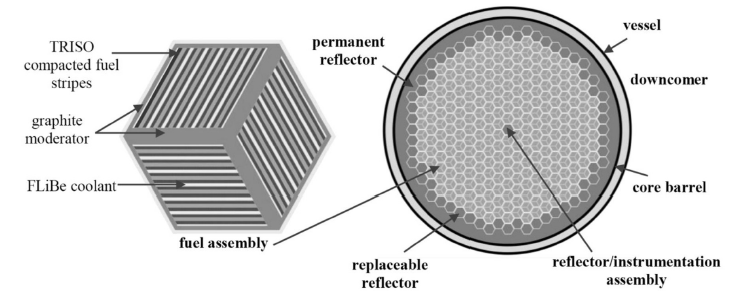
\includegraphics[width=0.9\linewidth]{ahtr.png} 
    \caption{FHR core configuration and fuel element \cite{ramey_monte_2018}.}
    \label{fig:ahtr}
\end{figure}

\subsection{Previous AHTR modeling efforts and challenges}
Modeling and simulation of the \gls{AHTR} design has been an ongoing effort 
since its conception in 2003 \cite{forsberg_molten-salt-cooled_2003}. 
The \gls{AHTR} core design differs significantly from the present \gls{LWR}-based 
nuclear power plants. 
These differences lead to modeling challenges and the need for verification and 
validation of modeling and simulation methods \cite{ramey_monte_2018}. 
Verification and validation of neutronics and thermal hydraulics tools' 
capability to successfully model the \gls{AHTR} design is a crucial step 
in support of licensure of the \gls{AHTR} design towards the eventual goal 
of deployment \cite{rahnema_phenomena_2019,rahnema_current_2015}. 
Several neutronic studies have been completed along the way to the current 
\gls{AHTR} design \cite{ramey_monte_2018,holcomb_fluoride_2013,greene_pre-conceptual_2010}. 
These efforts have shed light on the technical challenges facing the \gls{AHTR} design. 

In an effort to understand the challenges of \gls{FHR} materials, 
modeling the neutronics and thermal hydraulics in 
both plate and pebble fuelled \glspl{FHR}, a university-led Integrated 
Research Project \cite{zhang_integrated_2019} was conducted. 
During the research project, a panel of subject matter experts came together to 
generate a \gls{PIRT} by identifying phenomena and ranking their importance.
The \gls{PIRT} identifies areas in which additional research is needed to better 
understand important phenomena for adequate future modelling 
\cite{rahnema_phenomena_2019}. 
The phenomena identified as requiring further research are included in 
Table \ref{tab:phenomena}. 

\begin{table}[]
    \centering
    \onehalfspacing
    \caption{\gls{PIRT} identified \gls{FHR} physical phenomena requiring further research 
    \cite{rahnema_phenomena_2019}.}
	\label{tab:phenomena}
    \small
    \begin{tabular}{l|l}
    \hline
    \textbf{Category} & \textbf{Phenomena} \\ \hline
    Fundamental cross section data & - Moderation in FliBe \\
    & - Thermalization in FliBe \\
    & - Absorption in FliBe \\
    & - Thermalization in carbon \\
    & - Absorption in carbon \\ \hline
    Material Composition & - Fuel particle distribution \\ \hline
    Computational Methodology & - Solution Convergence \\ 
    & - Granularity of depletion regions \\
    & - Multiple heterogeneity treatment for generating multi-group \\ 
    & cross sections \\
    & - Selection of multi-group structure \\
    & - Boundary conditions for multi-group cross section generation \\ \hline 
    General Depletion & Spectral history \\ \hline 
    \end{tabular}
    \end{table}

The \gls{AHTR} has a complex core design due to the multiple heterogeneity present 
in the fuel introduced by presence of \gls{TRISO} particles embedded in plates 
\cite{ramey_monte_2018,rahnema_phenomena_2019}.
Accurately modeling the \gls{FHR}'s complex geometry with individual \gls{TRISO}
particle fidelity is necessary to obtain detailed reference power distributions 
to assess the accuracy of lower-fidelity models.
However, it is challenging, particularly for deterministic codes which 
use multigroup cross sections and traditional homogenization methods
\cite{ramey_monte_2018}. 
These traditional homogenization methods are insufficient to capture the correct physics 
in \glspl{FHR}, due to the multiple heterogeneity \cite{ramey_monte_2018}. 
In the \gls{AHTR}, single and multiple slab homogenization decreased computation time 
by 10, however they introduce a nontrivial error of $\sim$3\%
\cite{ramey_monte_2018,cisneros_neutronics_2012}.
Core physics parameters with acceptable uncertainty must be calculated to determine 
the feasibility and safety of the \gls{AHTR} design.
For Monte Carlo codes, statistical uncertainties must be reduced by increasing 
the number of neutron histories, however this comes at an increased 
computational cost.

Another technical challenge faced by the \gls{AHTR} design is the uncertainty of 
the graphite and carbonaceous moderator material properties: densities, temperatures
and thermal scattering data.
Also, the thermal scattering data ($S(\alpha,\beta)$ matrices) for the bound 
nuclei in the \gls{FLiBe} salt are lacking \cite{ramey_monte_2018}. 
Upon examination of the thermal scattering behavior of solid \gls{FLiBe}
\cite{mei_investigation_2013} and liquid \gls{FLiBe} \cite{zhu_thermal_2017}, 
it was observed that the bound and free atom cross section of \gls{FLiBe} are 
identical above 0.1eV and diverges below 0.01eV. 
This means that the use or absence of thermal scattering data will impact the 
accuracy of the results \cite{ramey_monte_2018}. 

\subsection{AHTR Benchmark}
In an effort to address and further understand the technical challenges described 
in the previous section, in 2019 the OECD-NEA initiated a benchmark to assess the 
state of the art modelling and simulation capabilities for \glspl{FHR} with 
\gls{TRISO} fuel embedded in fuel plates ("planks") of hexagonal fuel elements
\cite{noauthor_fluoride_nodate}. 
The benchmark plans to have three phases, starting from a single fuel element 
simulation without burnup, gradually extending to full core depletion and feedback. 
The overarching objective of the benchmark is to identify applicability, accuracy, 
and practicality of the current methods and codes to assess the current state 
of the art of \gls{FHR} simulation and modeling \cite{petrovic_preliminary_2021}. 
The benchmark also enables the cross-verification of codes and methodologies for the 
challenging \gls{AHTR} geometry, which is especially useful since applicable reactor 
physics experiments that may be used for validation of codes are scarce  
 \cite{petrovic_fhrahtr_2019,petrovic_preliminary_2021}. 
A detailed description of the phases of the benchmark and the results to date 
are described in Chapter \ref{chap:fhr-benchmark}. 

\section{Additive Manufacturing}
\gls{AM} is the formalized termed for what used to be called rapid prototyping 
and what is popularly called 3D printing \cite{gibson_additive_2014}. 
The basic principle of \gls{AM} is that a model is initially generated using a
\gls{3D CAD} system and is fabricated directly without the need for process 
planning. 
In \gls{AM}, the parts are made by adding materials in layers, each layer is a 
thin cross-section of the \gls{3D CAD} designed part, as opposed 
to subtractive manufacturing methods such as traditional machining
\cite{standard_standard_2012}. 
All commercialized \gls{AM} machines to date use a layer-based approach, and 
the major ways that they differ are in the materials that can be used, 
how the layers are created, and how the layers are bonded to each other
\cite{gibson_additive_2014}.
These major differences will determine the following factors: accuracy of the 
final part, its material and mechanical properties, time required to manufacture 
the part, the need for post-processing, size of \gls{AM} machine, overall 
cost of the machine and the process \cite{gibson_additive_2014}. 
Initially, \gls{AM} was used to manufacture prototypes. 
However, with improvements in material properties, accuracy and overall quality 
of \gls{AM} output, the applications for \gls{AM} expanded, to the 
current point in which some industries build parts for direct assembly purposes
\cite{uriondo_present_2015}.  
Furthermore, using \gls{AM} in conjunction with other technologies, such as 
high-power laser technology, has enabled the use of \gls{AM} technology 
to manufacture parts made from a variety of metals \cite{gibson_additive_2014}. 

\subsection{Application of Additive Manufacturing to Nuclear Reactor Core Components}
Many generation IV advanced reactor concepts have complex geometries, such as 
hex-ducts for sodium-cooled fast reactors, which are costly and difficult to 
fabricate using common processing techniques. 
These traditional processing routes also restrict the viable geometries for 
reactor designers \cite{sridharan_performance_2019}. 
Studies show the potential of using \gls{AM} for fabrication of nuclear fuel 
and core structural materials with complex geometries and at a lower cost. 
Without the geometric constraints of conventional fuel manufacturing, we can 
further optimize and improve fuel geometries to enhance fuel performance and 
safety \cite{bergeron_early_2018}. 

There has been experimental work done in the nuclear materials field towards 
demonstration of \gls{AM} of nuclear fuel and structural core materials. 
Bergeron et al \cite{bergeron_early_2018} successfully demonstrated additively 
manufacturing thorium dioxide using a stereolithography-based 3D printer 
and photopolymer resin. 
The high-density thorium dioxide objects were printed and sintered to densities 
of $\sim90\%$ \cite{bergeron_early_2018}. 
Rosales et al \cite{rosales_characterizing_2019} conducted a feasibility study 
of direct routes to fabricate dense uranium silicide ($U_3Si_2$) fuel pellets 
using the \gls{INL} invented \gls{AMAFT}. 
$U_3Si_2$ is an accident-tolerant nuclear fuel candidate due to its promising 
high uranium density and improved thermal properties. 
Its current metallurgical fabrication process is expensive and long, the goal of
\gls{AMAFT} is to fabricate $U_3Si_2$ at a lower cost, in a timely and
commercially-reliable manner \cite{rosales_characterizing_2019}.  
Sridharan et al \cite{sridharan_performance_2019} demonstrated the application of
the laser-blown-powder \gls{AM} process to fabricate \gls{FM} steel, a type of 
steel commonly used for cladding and structural components in nuclear reactors. 

% Takaaki_additive_2021

\section{Nuclear Reactor Design Optimization}
The practice of nuclear reactor optimization has been around since the conception of 
nuclear reactors. 
Optimization has been applied to nuclear reactor design, reactor reloading 
patterns, and the nuclear fuel cycle.  
% add some refs 
In the proposed work, we will focus on the optimization of nuclear reactor 
core design. 
The complexity of a nuclear reactor results in reactor design optimization 
being a multi-objective design problem requiring a tradeoff between desirable 
attributes \cite{byrne_evolving_2014,simon_sciences_2019}. 

Previous efforts towards nuclear reactor core design optimization include the use 
of deterministic and stochastic optimization techniques, evolutionary algorithms 
optimization, and these optimization methods coupled with surrogate models. 
Sacco et al \cite{sacco_two_2006,sacco_metropolis_2008} used stochastic 
optimization techniques such as the \gls{PCA} and Dueck's Great Deluge 
Algorithm (GDA), and a deterministic-stochastic hybrid optimization technique
that combined the \gls{PCA} with the deterministic Nelder–Mead Simplex algorithm
to optimize reactor dimensions, enrichment, materials etc., 
in order to minimize the average peak factor in a three-enrichment-zone reactor. 
Odeh et al \cite{odeh_core_2016} used the simulated annealing stochastic algorithm 
coupled with neutronics and thermal hyraulics codes, \gls{PARCS} and RELAP5, 
to develop an optimum core design for the \gls{NMR-50} to achieve a 10-year cycle length 
with minimal fissile loading. 
Kropaczek et al \cite{kropaczek_large-scale_2019} demonstrated the constraint 
annealing method, a highly scalable method based on the method of parallel 
simulated annealing with mixing of states \cite{kropaczek_constraint_2019}, for 
the solution of large-scale, multiconstrained problems in \gls{LWR} fuel cycle 
optimization. 
Peireira et al \cite{pereira_coarse-grained_2003,pereira_parallel_2008} 
used a coarse-grained parallel \gls{GA} and a niching \gls{GA}
to optimize the same problem as \cite{sacco_two_2006}. 
Kamalpour et al \cite{kamalpour_smart_2020} utilized the imperialist competitive 
algorithm, a type of evolutionary algorithm, to optimize a \gls{FCM} fuelled 
\gls{PWR} to extend the reactor core cycle length. 

There are multiple papers that utilize optimization methods with surrogate models 
to replace high fidelity neutronics or thermal hydraulics simulations that 
typically require a high computational cost. 
Kumar et al \cite{kumar_new_2015} combined genetic algorithm optimization 
with regression splines surrogate model to optimize a reactor model for 
high breeding of U-233 and Pu-239 in desired power peaking limits, desired 
keff using the following parameters: radius of a fuel pin cell, isotopic enrichment 
of the fissile material in the fuel, mass flow rate of the coolant, and temperature 
of the coolant at the core inlet.
Betzler et al \cite{betzler_design_2019} developed a systematic approach to 
build a surrogate model to serve in place of high-fidelity computational 
analyses, they then leveraged the surrogate model to generate optimized designs 
at a lower computational cost to understand the impact of design decisions on 
desired metrics for \gls{HFIR} \gls{LEU} core designs. 

\section{Evolutionary Algorithms}
Evolutionary algorithms have proved amenable to \gls{HPC} solution and 
scalable to tens of thousands of processors \cite{kropaczek_constraint_2019}